%%	SECCION documentclass																									 %%	
%%---------------------------------------------------------------------------%%
\documentclass[a4paper]{report}
%%---------------------------------------------------------------------------%%
%%	SECCION usepackage																											 %%	
%%---------------------------------------------------------------------------%%
\usepackage{amsmath, amsthm}
\usepackage{amsfonts}%
\usepackage{amssymb}%
\usepackage[spanish,activeacute]{babel}
\usepackage{caratula}
\usepackage{hyperref} %para que haya hiperv�nculos
\usepackage{graphicx} % Para el logo magico!
\usepackage[latin1]{inputenc}
\usepackage{color}
\usepackage{ingsoft1}
\usepackage{slashbox} %Para agregar divisione en diagonal en las tablas
\usepackage{alltt} % que es este paquete???
 \usepackage{pdflscape}%Para poner paginas apaisadas


\newcommand{\rojo}[1]{\textcolor{red}{#1}}
\newcommand{\azul}[1]{\textcolor{blue}{#1}}
\newcommand{\verde}[1]{\textcolor{green}{#1}}
\newcommand{\descripcion}[1]{\rojo{#1}}
\newcommand{\ejemplo}[1]{\azul{\begin{quote} #1 \end{quote}}}
\newcommand{\comentario}[1]{\rojo{\emph{#1}}}
%\newcommand{\definicion}[1]{\textbf{#1}}

\newtheorem{theorem}{Theorem}
\newtheorem{definicion}[theorem]{Definici�n}

%%---------------------------------------------------------------------------%%
%%	SECCION opciones																												 %%	
%%---------------------------------------------------------------------------%%

\oddsidemargin 0cm
\headsep -1.4cm
\textwidth=16.5cm
\textheight=23cm
\makeindex

%%---------------------------------------------------------------------------%%
%%	SECCION document	                                                       %%	
%%---------------------------------------------------------------------------%%
\begin{document}
	\setcounter{page}{0} %para que numere a la caratula como p�gina 0 y a las demas a partir de 1

%%---- Caratula -------------------------------------------------------------%%
\title{Resumen Final}
\author{Santiago Avenda�o\thanks{This is for making an acknowledgement.}
\\Universidad de Buenos Aires, Argentina}
\date{10 Febrero, 2009}

\materia{Resumen Final}
\titulo{Ingenier'ia de Software I}
%\subtitulo{}

\integrante{Avenda\~no, Santiago}{113/06}{santiavenda2@hotmail.com}
\grupo{Grupo n'umero}
%\resumen{}
\maketitle

\tableofcontents

\newpage
%% Based on a TeXnicCenter-Template by Tino Weinkauf.
%%%%%%%%%%%%%%%%%%%%%%%%%%%%%%%%%%%%%%%%%%%%%%%%%%%%%%%%%%%%%

%%%%%%%%%%%%%%%%%%%%%%%%%%%%%%%%%%%%%%%%%%%%%%%%%%%%%%%%%%%%%
%% PDF-Informations
%%%%%%%%%%%%%%%%%%%%%%%%%%%%%%%%%%%%%%%%%%%%%%%%%%%%%%%%%%%%%
%%
%% ATTENTION: You need a main file to use this one here.
%%            Use the command "\input{filename}" in your
%%            main file to include this file.
%%

\pdfinfo{                               % Info dictionary of PDF output;
                                        % all keys are optional.
    /Author (Santiago Avendano)
    /CreationDate (D:20090210195001)    % (D:YYYYMMDDhhmmss)
                                        % YYYY  year
                                        % MM    month
                                        % DD    day
                                        % hh    hour
                                        % mm    minutes
                                        % ss    seconds
                                        %
                                        % default: the actual date
                                        %
    /ModDate (D:default)         % ModDate is similar
    /Creator (Santiago Avendano)               % default: "TeX"
    /Producer (pdfTeX)                  % default: "pdfTeX" + pdftex version
    /Title (Ingenieria de Software 1 - Resumen final)
    /Subject (Ingenieria de Software)
    /Keywords (Requerimientos, Modelos, Disenio, Testing)
}

\clearpage

\newpage
%Secci�n: Introducci�n Ingenier�a de Software

\chapter{Ingenier�a de Software}
\section{Introducci�n}
\subsection{Definici�n}

La \emph{Ingenier�a de Software} es la aplicaci�n de un acercamiento sistem�tico, disciplinado y cuantificable para el desarrollo, operaci�n y mantenimiento de un software.

La Ingenier�a de Software(IS) re�ne conocimientos, herramientas y m�todos para definir requerimientos de software y realizar dise�o, construcci�n, testing y mantenimiento de software.

\subsubsection{Objetivo:} Se ocupa de construir un producto de software de buena calidad, lidiando con m�ltiples restricciones (tiempo, presupuesto, requerimientos, etc)

\subsubsection{Problem�ticas:}
\begin{itemize}
	\item Lidiar con la escala y complejidad de sistemas de software
	\item Identificar que significa buena calidad
	\item Disciplina joven, v�ctima de su propio �xito
\end{itemize}

\section{Ciclo de Vida de Desarrollo de Software}

\subsection{Modelo Cascada (Royce, 1970)}

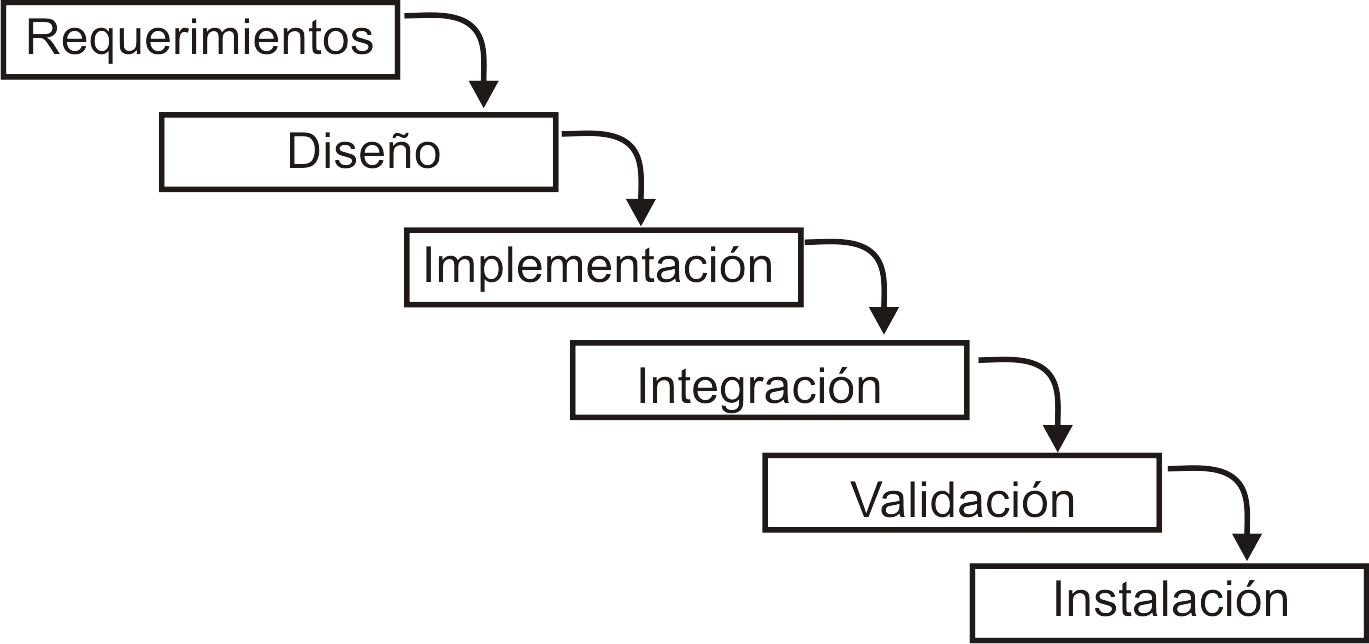
\includegraphics[width = 0.9\textwidth]{Graficos/ModeloCascada.png}

\subsection{Modelo V}

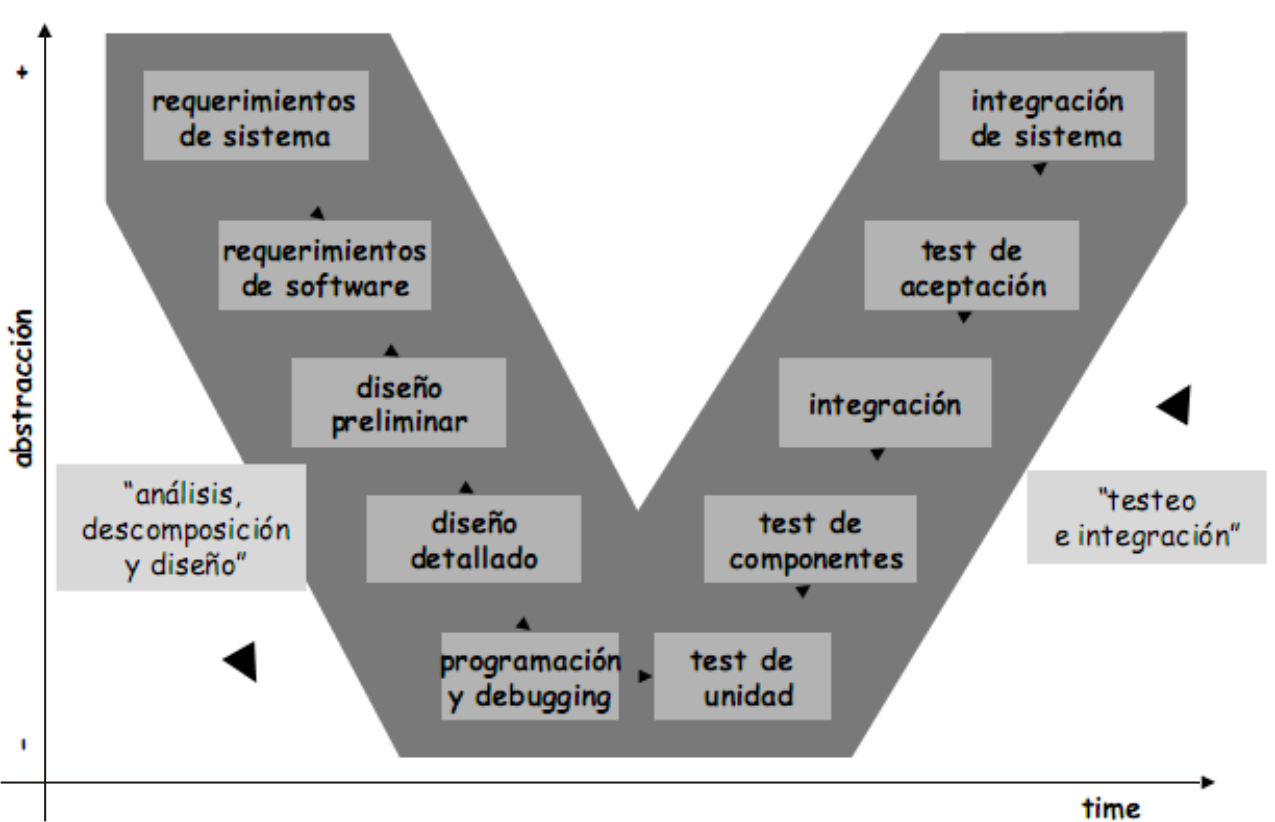
\includegraphics[width = 0.9\textwidth]{Graficos/ModeloV.png}

\subsection{Modelo Espiral (Boehm,1988)}

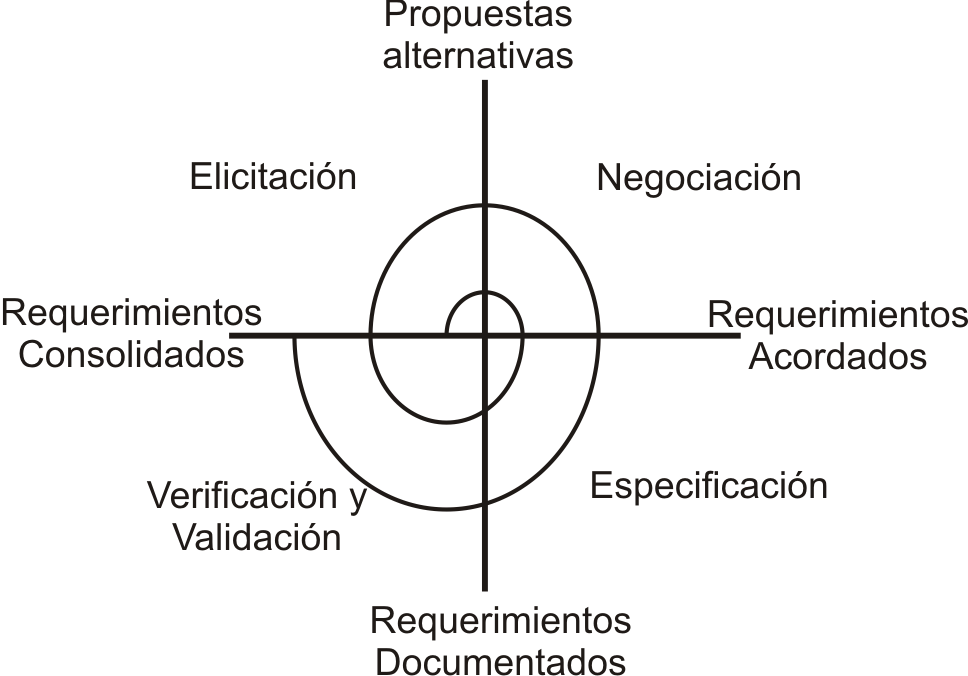
\includegraphics[width = 0.9\textwidth]{Graficos/ModeloEspiral.png}

\newpage

\subsection{Unified SW Development Process (Jacobson, 1999) }

Divisi�n en fases e iteraciones

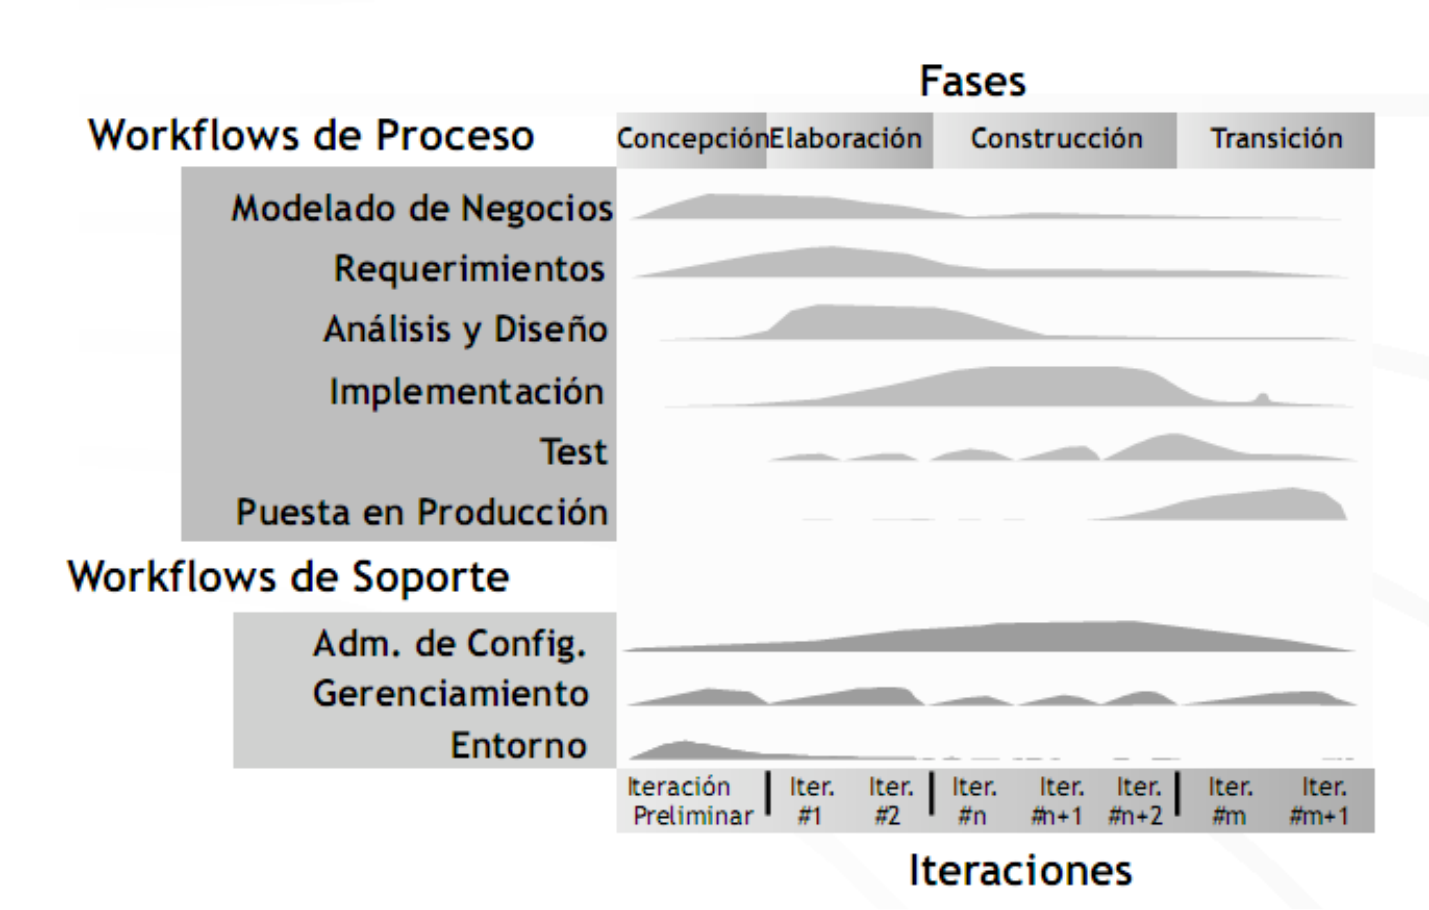
\includegraphics[width = 0.9\textwidth]{Graficos/ModeloJacobson.png}

\subsection{Modelo Twin Peaks}

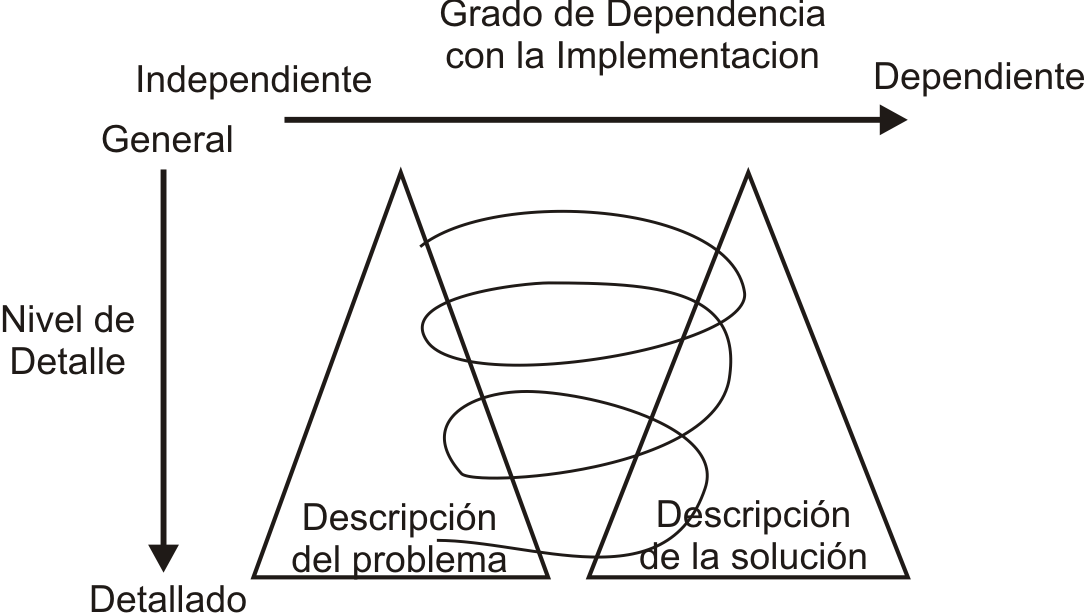
\includegraphics[width = 0.9\textwidth]{Graficos/ModeloTwinPeaks.png}

\newpage

\section{Modelos}

Un \emph{modelo} es una representaci�n de la realidad.

Los modelos son construidos con el objetivo de lidiar con la complejidad de los sistemas.

Los modelos son efectivos porque:

\begin{itemize}
	\item Describen un aspecto del problema a resolver
	\item Omiten detalles no relevantes al an�lisis para el cual se construye el modelo
	\item Permite comunicar en forma precisa aspectos del problema y la soluci�n a otras personas.
	\item Son m�s baratos de construir
	\item Facilita el an�lisis (permite detectar errores y falencias tempranamente)
\end{itemize}

Los modelos tienen un Scope y un Span

\begin{description}
	\item[Scope(aspecto):] tipo de fen�meno que se capta
	\item[Span(segmento):] individuos descriptos
\end{description}

\emph{Los modelos en Ingenier�a de Software son lenguajes formales con una denotaci�n precisa en el mundo real}


Los lenguajes formales tienen:

\begin{itemize}
	\item una \emph{sintaxis}(gr�fica/texto) para describirlos: cu�les son los garabatos permitidos
	\item una \emph{sem�ntica} para abstraer accidentes sint�cticos: cu�les de estos garabatos significan lo mismo.
\end{itemize}

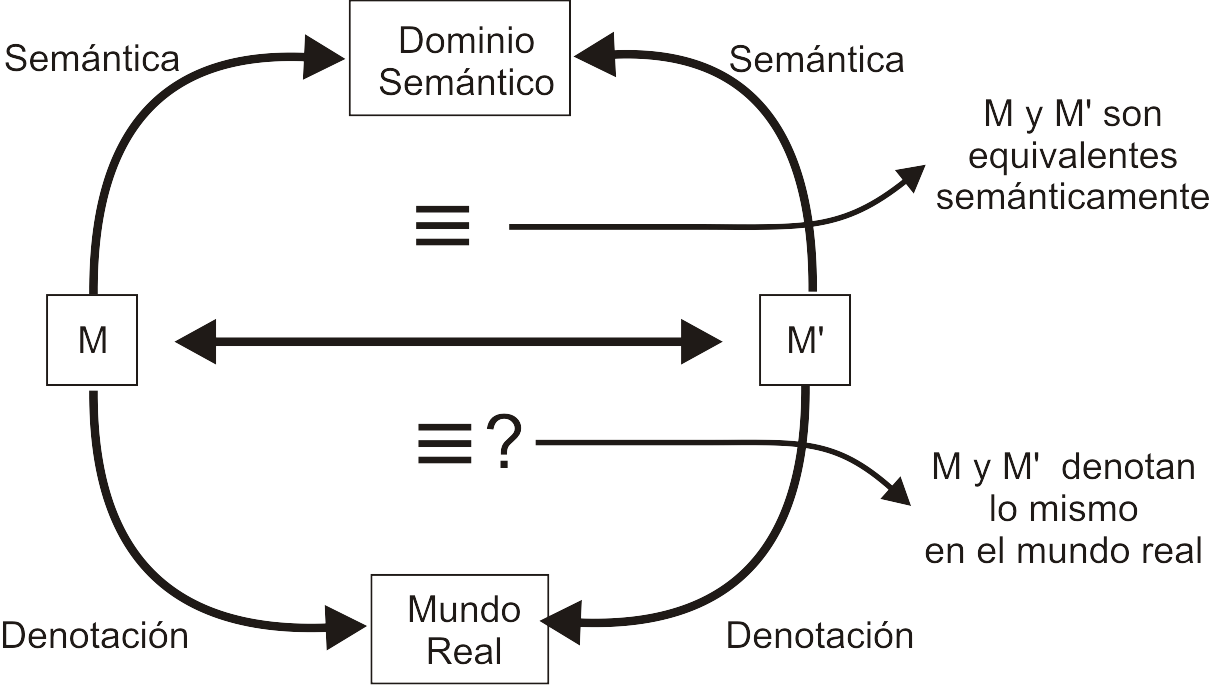
\includegraphics[width = 0.9\textwidth]{Graficos/Modelos.png}

Un sistema se analiza desde m�ltiples modelos complementarios. Cada modelos enfoca una aspecto(scope) del sistema, para permitir an�lisis rigurosos y escalables.

Es imposible vincular los distintos modelos formalmente, manteni�ndolos analizables y entendibles(�tiles).

Ejemplos de modelos: de Objetivos, de Agentes, de Operaciones, Conceptuales, de Comportamiento, Arquitect�nicos.

\newpage

\section{Validaci�n y Verificaci�n}
\label{VerificacionValidacion}
\begin{description}
	\item[Validaci�n:] $\longrightarrow$ Mundo vs. Modelo
	Proceso cuyo objetivo es \emph{incrementar la confianza} de que una descripci�n formal \emph{se corresponde} con la realidad. Es imposible de realizar.
	\item[Verificacion:] $\longrightarrow$ Modelo vs. Modelo
	Proceso cuyo objetivo es \emph{garantizar} que una descripci�n formal \emph{es correcta} con respecto a otra.
\end{description}

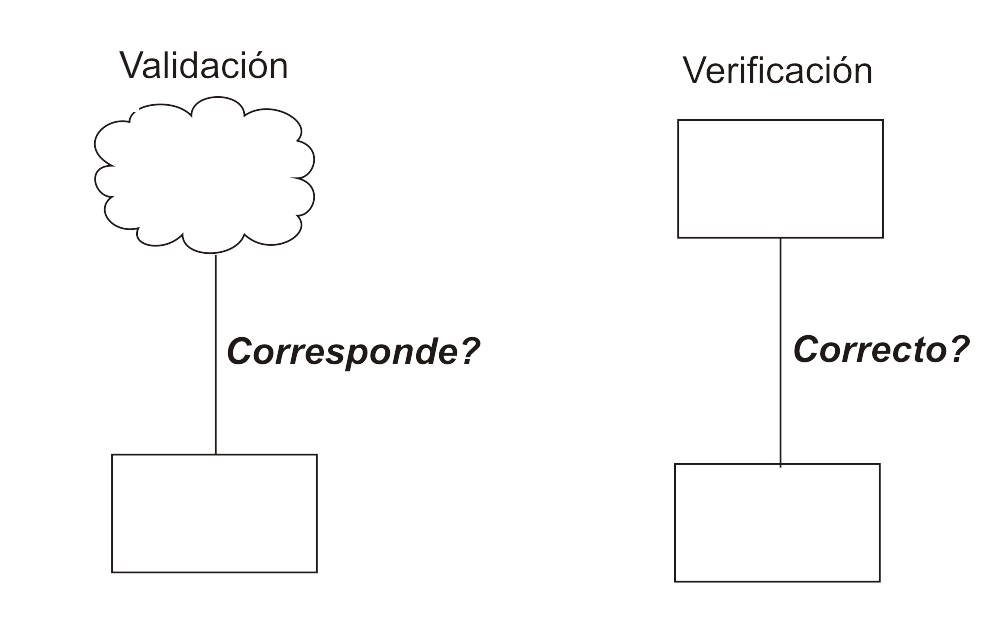
\includegraphics[width = 0.9\textwidth]{Graficos/VerificacionValidacion.png}

\section{Resumen}

\begin{itemize}
	\item Que es la IS? Definici�n, objetivos, problemas
	\item Ciclo de vida de desarrollo de Software
	\item Modelos: definici�n, ventajas	
		\begin{itemize}
			\item Scope y Span
			\item Sintaxis, Sem�ntica y Denotaci�n
			\item Verificaci�n y Validaci�n
		\end{itemize}
\end{itemize}
\clearpage

\newpage
%Cap�tulo 2: Ingenir�a de Requerimientos

\chapter{Ingenier�a de Requerimientos}

\section{Introducci�n}

\subsection{Definici�n}

Todo Software se desarrolla con un \emph{prop�sito}. Luego podemos definir \emph{calidad} como el grado con que el software cumple con el prop�sito.

La \emph{\textbf{Ingenier�a de Requerimientos (RE)}} es un conjunto de actividades concernientes a identificar y comunicar el prop�sito de un sistema intensivo de software y el contexto en que ser� usado. 

Tanto el problema como la soluci�n son el resultado del comportamiento emergente de la interacci�n entre los componentes del sistema. Por eso hablamos de Ingenier�a de Requerimientos de \emph{Sistemas Intensivos en Software} (Software + Hardware + Entorno).

Por lo tanto la Ingenier�a de Requerimientos act�a como puente entre las necesidades del mundo real de los usuarios, clientes y otros individuos afectados por el sistema de software, y las capacidades y oportunidades surgidas a partir de las tecnolog�as de software intensivo.

\subsection{Separaci�n del problema y la soluci�n}

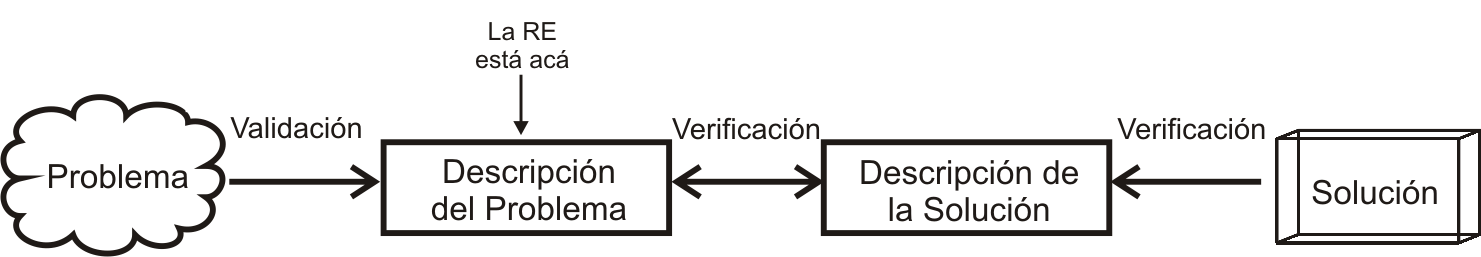
\includegraphics[width = 0.9\textwidth]{Graficos/separacion.png}

La Ingenier�a de Requerimientos requiere controlar que:

\begin{itemize}
	\item El problema se corresponde con lar verdaderas necesidades (validaci�n)
	\item La soluci�n correctamente resuelve la descripci�n del problema (verificaci�n)
\end{itemize}

\subsection{Actividades de Ingenier�a de Requerimientos}

\begin{description}
	\item[Elicitaci�n:] evocar una respuesta de alguien como reacci�n a preguntas o acciones.
	\item[Modelado:] documentar rigurosamente para an�lisis (abstraer y estructurar lo elicitado)
	\item[An�lisis:] verificaci�n inter e intra modelos
	\item[Validaci�n:] �los modelos se corresponden con la realidad?
	\item[Priorizaci�n:] establecer criterios de preferencia con respecto a alcance y objetivos.
	\item[Negociaci�n:] unificar criterios entre los interesados
	\item[Especificaci�n:] documentaci�n completa y detallada (documento final) 
\end{description}

\section{Modelo de Jackson}
\comentario{completar}

\section{Modelo de las 4 variables}
\comentario{completar}

\section{Diagrama de Contexto}
\comentario{completar}

\section{Modelo de Objetivos}
\comentario{completar}

\section{Modelo de Operaciones}
\comentario{completar}

\section{Modelo Conceptual}
\comentario{completar}

\section{Modelos de Comportamiento}
\comentario{completar}

\clearpage


\newpage
%Secci�n Dise�o

\chapter{Dise�o}
\section{Definici�n}

\noindent Dise�ar involucra estructurar la soluci�n utilizando abstracciones y relaciones entre las abstracciones para:
\begin{itemize}
	\item Documentar y comprender la propuesta de soluci�n
	\item Razonar sobre su grado de adecuaci�n a los requerimientos
	\item Comunicarla e implementarla
	\item Verificar/Validar el producto final
	\item Modificar/Adaptar la soluci�n cuando cambien los requerimientos
\end{itemize}

\noindent A diferencia de requerimientos, en dise�o:
\begin{itemize}
	\item Se denotan conceptos del mundo de la soluci�n y no del problema, pero incluye fen�menos de la interfaz mundo-m�quina.
	\item Se describe propiedades localizadas (unidad, componente, m�dulo) y son de naturaleza operacional.
\end{itemize}

\subsubsection*{Objetivos de la etapa de dise�o}
\begin{itemize}
	\item Descomponer el sistema en entidades de dise�o ``m�s chicas''
	\item Determinar la relaci�n entre entidades
	\item Fijar mecanismos de interacci�n
	\item Especificar interfaces y funcionalidades de entidades
	\item Identificar oportunidades para el reuso
	\item Documentar lo anterior y los fundamentos de las elecciones
\end{itemize}

El dise�o es un proceso iterativo, enfocado al \emph{``que y c�mo''} ( en contraposici�n al \emph{``que y porque''} de la etapa de relevamiento de Requerimientos).

\section{Vistas}
La descripci�n de un sistema complejo no es unidimensional. Es clave saber cu�les son las vistas relevantes y vinculadas. 

Las vistas enfatizan aspectos e ignoran otros para que el problema sea abordable. Cada vista enfoca en una problem�tica en particular, permite responder cierta clase de preguntas y admite varios niveles de abstracci�n y t�cnicas de modelado.

Los diferentes tipos de vistas pueden clasificarse en
\subsection{Vista Est�tica o Modular} 

Relacionada con el agrupamiento de c�digo
	
	\textbf{M�dulo:} unidad de c�digo que implementa un conjunto de responsabilidades (una clase, una colecci�n de clases o cualquier descomposici�n de c�digo). Es una unidad \emph{design-time}.
	
	\subparagraph{Entidades:} m�todos, procedimientos, clases, librer�as, DLLS, APIs, paquetes. m�dulos.
	\subparagraph{Relaciones:} es-parte-de, depende-de, es-un.
	\subparagraph{Ejemplos:} diagrama de clases, diagrama de paquetes.

La manera de modularizar suele determinar caracter�sticas como: modificabilidad, portabilidad y reuso.

\noindent An�lisis que permite realizar:
\begin{itemize}
	\item Trazabilidad de requerimientos
	\item An�lisis de impacto
	\item Comunicaci�n a otras personas
	\item Nivel de granularidad
\end{itemize}

\noindent No sirve para:
\begin{itemize}
	\item realizar inferencias sobre comportamiento del sistema en su ejecuci�n
	\item realizar an�lisis de performance.
\end{itemize}


\subsection{Vista Din�mica o de Componentes y Conectores}

Relacionada con las entidades \emph{run-time}.

\textbf{Entidades:} procesos, threads, objetos, protocolos.

Las entidades \emph{run-time} son instancias de tipos de conector o componente. Son entidades que consumen recursos y contribuyen al comportamiento en ejecuci�n del sistema.

\textbf{Relaciones:} se-comunica-con, bloquea, contiene, crea, destruye.

\textbf{Ejemplos:} m�quinas de estado, diagrama de secuencias y colaboraci�n, diagrama de objetos, diagrama de componentes.

\noindent An�lisis que permite realizar:
\begin{itemize}
	\item Confiabilidad
	\item Performance: tiempo de respuesta, tiempo de latencia y volumen de procesamiento
	\item Recursos requeridos: almacenamiento y procesamiento
	\item Funcionalidad
	\item Protocolos
	\item Seguridad
\end{itemize}

\subsection{Vista de Despliegue (Deployment)}

\textbf{Entidades:} recursos y repositorios

\textbf{Relaciones:} procesos ejecuta sobre server, c�digo de m�dulos almacenado en directorios, equipo de trabajo desarrolla paquete.

\textbf{Ejemplos:} Diagrama de Despliegue

\section{Principios de Dise�o}

\subsection{Descomposici�n}

\emph{Divide and conquer:} se parte cada parte del problema en subproblemas o componentes m�s peque�os siguiendo una estrategia adecuada (como ser pasos de ejecuci�n, datos, tiempos, funcionalidades, etc), determinar las relaciones entre dichos componentes e iterar. 

Es importante tener una estrategia de composici�n, no s�lo de divisi�n (Divide to Conquer and reunite to rule)

\subsection{Abstracci�n}
Se basa en suprimir detalles de la implementaci�n y posponer decisiones de dise�o que ocurren a distintos niveles del an�lisis. El objetivo es simplificar el an�lisis, comprensi�n y justificaci�n de decisiones.

La abstracci�n puede ser procedural (funciones, m�todos, etc), de datos (TADs) o de control (loops, iteradores, multitasking).

\subsection{Encapsulamiento}
	Se basa en mantener una clara separaci�n entre interface e implementaci�n. Con esto se logra no conocer ni usar m�s de lo que la interfaz promete.
	
	\subparagraph{Control Inversion Principle:} Uso de frameworks, implementaciones parciales que el usuario debe rellenar para lograr la funcionalidad deseada; la diferencia principal con las librer�as es que es el framework el que invoca el c�digo del usuario y no al rev�s.

\subsection{Information Hiding}

Relacionado estrechamente con encapsulamiento.

Se base en esconder decisiones de dise�o que pueden llegar  a cambiar. Con esto se busca minimizar el impacto de cambios futuros. Para esto se programa orientado a interfaces.

\subparagraph{Dependency Inversion Principle:} Las dependencias se hacen hacia interfaces o clases abstractas, no hacia las implementaciones concretas.


\subsection{Modularidad}
Un m�dulo es una entidad est�tica que agrupa ciertas funcionalidades (superior a una clase). Tiene una interfaz bien separada de su implementaci�n, garantiza alta cohesi�n y bajo acoplamiento.

Indicios de una buena modularizaci�n es tener una jerarqu�a de m�dulos lo suficientemente independientes, con responsabilidades claras y delimitadas, donde un cambio en uno impacta lo menos posible en el resto del sistema.

\paragraph{Cohesi�n:}

Es el grado de uni�n (cu�n bien trabajan juntos) que tienen los distintos elementos de un m�dulo. Alta cohesi�n provee: robustez, confiabilidad, reusabilidad, comprensibilidad, testeabilidad y mantenibilidad.

Pueden definirse distintos tipos de cohesi�n, de peor a mejor, consider�ndose aceptables s�lo los tres �ltimos:
\begin{itemize}
	\item \textbf{Coincidental:} Ej. mis funciones de uso frequente, utils.lib
	\item \textbf{L�gico:} existe una categor�a l�gica que agrupa elementos aunque hagan cosas muy distintas (ej. todas las rutinas de I/O)
	\item \textbf{Temporal:} agrupadas por el momento en que se ejecutaran (ej. funciones que atajan un error de output, crean un error en un log y notifican al usuario)
	\item \textbf{Procedural:} agrupadas por pertenecer a una misma secuencia de ejecuci�n o pol�tica (ej. funciones que chequean permisos y abren archivos)
	\item \textbf{Comunicacional:} agrupadas por operar sobre los mismo datos (ej. objetos, operaciones sobre clientes)
	\item \textbf{Secuencial:} agrupadas porque el output de uno es el input de otro
	\item \textbf{Funcional:} agrupadas porque contribuyen a una tarea bien definida del m�dulo
\end{itemize}

\subparagraph{Single Responsibility Principle:} A class should have only one reason to change; busca obtener un alto grado de cohesi�n, una clase debe tener una y solo una responsabilidad.

\paragraph{Acoplamiento:}

Grado de dependencia del m�dulo sobre otros m�dulos y en particular las decisiones de dise�o que estos hacen. Generalmente proporcional al grado de cohesi�n. 

Un alto acoplamiento conlleva una alta propagaci�n de cambios y necesidades de testing, dificulta la comprensi�n de los m�dulos de forma aislada y trae problemas al reuso y retesteo.

Los tipos de acoplamiento son, de mayor a menor:

\begin{itemize}
	\item \textbf{Contenido:} Cuando un m�dulo modifica o conf�a en el lo interno de otro
	\item \textbf{Com�n:} Cuando comparten datos comunes 
	\item \textbf{Externo: }Cuando comparten aspectos impuestos externamente al dise�o (ej. formato de datos, protocolo de comunicaci�n, interfaz de dispositivo)
	\item \textbf{Control:} Cuando un m�dulo controla la l�gica del otro 
	\item \textbf{Estampillado(Stamp):} Cuando comparten una estructura de datos pero cada uno usa s�lo una porci�n 
	\item \textbf{Datos:} M�dulos se comunican a trav�s de datos en par�metros 
	\item \textbf{Mensajes: }M�dulos se comunican a trav�s de mensajes, posiblemente no se conocen expl�citamente
\end{itemize}

\subparagraph{Interface Seggregation Principle:} muchas interfaces para los diferentes clientes son mejores que una �nica interface de prop�sito general. Busca separar interfaces para minimizar dependencias y reducir el fanning.

\subsection{Extensibilidad}

El dise�o debe ser capaz de acomodarse a los cambios de requerimientos sin sufrir modificaciones, siendo extendido con facilidad.

\subparagraph{Open/closed Principle:} la entidades de software deben ser abiertas para la extensi�n  pero cerradas para la modificaci�n be open. Suele implementarse mediante polimorfismo e interfaces.

\subparagraph{Liskov Substitution Principle:} las subclases deben ser sustituibles por sus clases bases.

\subparagraph{Ley de Demeter:} No hablar con extra�os, se basa en que un m�todo de un objeto s�lo puede llamar m�todos del propio objeto, sus par�metros o aquellos objetos que constituyen el objeto de manera directa o fueron creados por �l. Se evita llamar m�todos de objetos remotos retornados por otros m�todos. 

Facilita la mantenibilidad y adaptabilidad pero tiende a generar wrappers molestos y poco cohesivos.

\section{Programaci�n Orientada a Objetos(POO)}
\subsection{Definiciones}

\textbf{Objeto:} entidad \emph{run-time} que act�a como una unidad de encapsulamiento. Encapsula estado (v�a variables internas) y comportamiento (v�a m�todos internos).

Los objetos encapsulan atributos/campos permitiendo acceso a ellos �nicamente a trav�s de los m�todos.

\textbf{Clase} entidad \emph{design-time}\footnote{No es estrictamente verdad, depende del leguaje (Ej: en Smaltalk las clases son objetos)}. Representa una clasificaci�on de objetos. Define el comportamiento y atributos de un grupo de objetos con estructura y comportamiento similar (un objeto es una instancia de una clase).

La \emph{instanciaci�n} es el proceso de creaci�n de un objeto a partir de la definici�n de una clase. Se realiza mediante el llamado a un constructor.

\subsection{Relaciones entre clases}
\begin{itemize}
	\item \textbf{Dependencia:} define una relaci�n \emph{``usa''} o \emph{``conoce a''}. Indica que el cambio de una clase puede afectar a la otra. Es la relaci�n m�s d�bil.
	\item \textbf{Agregaci�n:} indica una relaci�n \emph{``parte de''} o \emph{``tiene un''}. Es un tipo especial de dependencia.
	\item \textbf{Composici�n:} es un tipo especial de agregaci�n donde:
		\begin{itemize}
			\item las partes no se comparten
			\item la existencia de las partes depende de la existencia del contenedor.
		\end{itemize}
	\item {Generalizaci�n/Especializaci�n (Herencia):} denota la relaci�n \emph{``es un''}		
		\begin{itemize}
			\item Permite reuso y factorizaci�n de c�digo
			\item Permite polimorfismo por medio de subtipado
			\item Es el mecanismo de extensi�n sugerido por medio de subtipado
		\end{itemize}
\end{itemize}

\subsection{Polimorfismo}
Se refiere a tratar de manera uniforme estructuras que pueden tener m�s de un forma.

\paragraph{Conceptos relacionados:}
\begin{itemize}
	\item \emph{Herencia:} es el proceso de derivar una clase especializada de una clase ya existente.
	\item \emph{tipo real(actual):} es el tipo que tiene un objeto en run-time (\texttt{new relojDigital})
	\item \emph{tipo aparente:} es el tipo que deriva est�ticamente del compilador (\texttt{Reloj r})		
		\begin{itemize}
			\item \emph{Regla: el tipo aparente debe ser supertipo del tipo real.}
		\end{itemize}
	\item \emph{Binding:} resoluci�n del m�todo invocado (si es Late-Binding se hace en tiempo de ejecuci�n)
	\item \emph{Upcasting} y \emph{Downcasting}
\end{itemize}

\subsection{Clase vs. Tipo}

Un \textbf{tipo} $T$ denota un conjunto de objetos que satisface un predicado asociado al tipo $T$.

Un \textbf{subtipo} $S$ de $T$ denota un subconjunto de elementos de $T$ que satisfacen un predicado m�s restrictivo que asociado al tipo $T$.

\paragraph{Principio de Sustituci�n de Liskov/Wing}
\emph{Cualquier propiedad que podamos probar sobre objetos del tipo/clase $T$, tambi�n debe poder probarse para objetos del subtipo $S$.}

Es una manera razonable de lograr subtipado sano en jerarqu�as de clases OO (algunos programadores lo encuentran muy restrictivo)

Significa que las subclases preservan el comportamiento de las superclases.

El requerimiento se cumple si pedimos \textbf{contravarianza} en los argumentos y \textbf{covarianza} en los resultados.

\comentario{Poner grafico de Liskov}

\subsection{Clases Abstractas e Interfaces}

Una \textbf{Clase Abstracta} es una clase que no puede ser instanciada. Agrupa una implementaci�n com�n a un conjunto de clases. No dan una implementaci�n concreta (m�todos abstractos).

Una \textbf{interface}(Java) es un conjunto de m�todos y constantes identificadas con un nombre. Los m�todos de una interface no son implementados por ella. Las clases (abstractas o no) derivadas de una interface, deben implementar todos los m�todos de la interface.

Las interfaces son utilizadas para separar (desacoplar) la especificaci�n disponible al usuario de las implementaciones. Adem�s se puede ``simular'' herencia m�ltiple haciendo que una clase implemente dos interfaces.

\section{Patrones de Dise�o}
\comentario{completar}







\clearpage

\newpage
%section Testing
\chapter{Testing}
\section{Verificaci�n}
Recordemos algunos conceptos \footnote{ver \ref{VerificacionValidacion}}
\begin{description}
\item [Validaci�n:] proceso cuyo objetivo es \emph{incrementar la confianza} de que una descripci�n formal se \emph{corresponde} con la realidad.
\item [Verificaci�n:] proceso cuyo objetivo es \emph{garantizar} que una descripci�n formal es \emph{correcta} con respecto a otra.
\end{description}

La verificaci�n plantea la pregunta: �Estamos haciendo el producto correctamente? (en relaci�n con un componente anterior que describe nuestro producto)

\begin{description}
	\item [Verificaci�n Din�mica:] consiste en ejecutar y observar el comportamiento de un producto.	
	\begin{itemize}
		\item Testing
		\item Run time monitoring
		\item Run time verification
	\end{itemize}
	
	\item [Verificaci�n Est�tica:] consiste en realizar un an�lisis de una representaci�n est�tica del sistema para descubrir problemas.
	\begin{itemize}
		\item Inspecciones, Revisiones, Walkthrough (seguimiento)
		\item An�lisis de Reglas Sint�cticas sobre c�digo
		\item An�lisis Data Flow sobre c�digo
		\item Model Checking
		\item Prueba de teoremas
	\end{itemize}
\end{description}

\section{Calidad de Software}
\textbf{Conceptos relacionados:} Confiabilidad, Usabilidad, Correcci�n, Robustez, Facilidad de Mantenimiento, Seguridad, Reusabilidad datos, Verificabilidad + Claridad, Funcionalidad, Interoperabilidad.

La calidad del producto depende de tareas realizadas durante todo el proceso de desarrollo. Detectar errores en forma temprana ahorra esfuerzos, tiempo, recursos.

\subsection*{Definiciones}
\begin{description}
	\item [Falla:] diferencia entre los resultados esperados y reales (manifestaci�n de un defecto).
	\item [Defecto:] est� en el texto del programa, una especificaci�n, un dise�o, y desde all� se hace visible una falla.
	\item [Error:] equivocaci�n humana.
\end{description}

Un error lleva a uno o m�s defectos. Un defecto lleva a 0, 1 o m�s fallas.

\section{Testing}
\textbf{Definici�n:} verificaci�n din�mica de la adecuaci�n del sistema a los requerimientos (de distinto tipo). Es el proceso de ejecutar un producto para verificar que satisface los requerimientos e identificar diferencias entre el comportamiento real y el comportamiento esperado. 

\textbf{No prueba la correctitud del software!!!} 

\begin{quote}
El testing puede demostrar la presencia de errores, nunca su ausencia (Dijkstra)
\end{quote}

El objetivo del proceso de Testing es encontrar fallas importantes del sistema

Se realiza ejecutando el programa y comparando resultados contra un or�culo (el mismo tester) \footnote{Se asume que se puede ejecutar el programa, que se conoce el resultado esperado y que el resultado esperado puede compararse con el resultado obtenido.}.

\subsection{Proceso de testing}
El testing debe ser un proceso paralelo al desarrollo, no una actividad al final.

\subsubsection{Niveles de test}

\begin{description}
	%\item Aceptaci�n: �ltimo test que se hace junto con el cliente
	\item [Test de Sistema:] testea la funcionalidad del sistema completo con respecto a lo requerido por el cliente. Si el cliente participa se lo denomina \textbf{Test de aceptaci�n}.
	\item [Test de Integraci�n:] test orientado a verificar que las partes de un sistema, que funcionan bien aisladamente, tambi�n lo hacen en conjunto
	\item [Test de Unidad:] test realizado sobre una unidad de c�digo peque�a y claramente definida (m�todo, procedimiento, etc). Com�nmente es realizado por los desarrolladores.
\end{description}

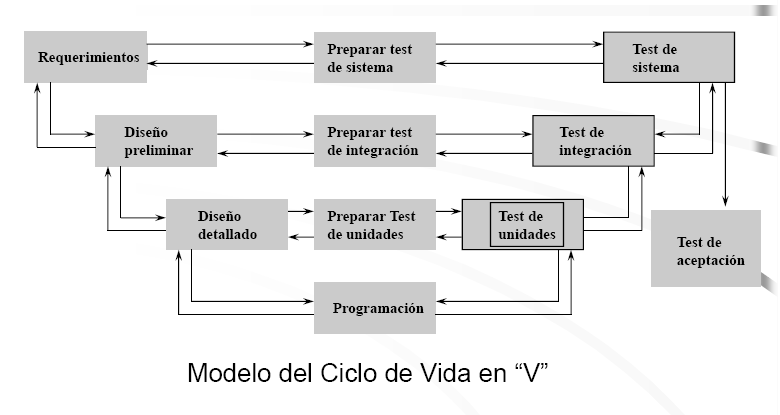
\includegraphics[width = 0.9\textwidth]{Graficos/procesoTesting.png}

El \textbf{el test funcional o de sistema} se prepara inicialmente en funci�n de los requerimientos. Luego este test dar� lugar al \textbf{test aceptaci�n}.

Sobre la base anterior se realiza un dise�o preliminar que incluye al \textbf{test de integraci�n}, y el dise�o detallado el \textbf{test de unidades}. Una vez todo listo se comienza con la programaci�n.

Asociado a la implementaci�n de los tests, est� la creaci�n del ambiente, la ejecuci�n de los casos, la documentaci�n, el seguimiento, etc.

\subsubsection{Actividades del proceso de Testing}
 Asociadas a arquitectura y dise�o detallado

\begin{itemize}
	\item Planificaci�n de test de integraci�n y unidad
	\item Generaci�n de casos de test funcionales
\end{itemize}

 Asociadas a la implementaci�n 
\begin{itemize}
	\item creaci�n de ambiente de ejecuci�n de tests
	\item generaci�n de casos de test estructurales
	\item ejecuci�n de test de unidad
	\item ejecuci�n de test de integraci�n
	\item documentaci�n de resultados
	\item seguimiento de errores
	\item test de regresi�n
\end{itemize}

\subsection{Terminolog�a}
\begin{description}
	\item[Requerimientos de Test:] qu� quiero testear.
	\item[Especificaciones de Test:] supuestos y definiciones que sirven para generar los casos de test para el requerimiento de test.
	\item[Casos de Test:] descripciones de condiciones o situaciones a testear.
	\item[Dato de Test:] asignaci�n de valores concretos de par�metros para ejecutar un caso de test.
	\item[Test Suite:] conjuntos de datos de test con los que se testea el programa.
\end{description}

Un test suite $T$ es \emph{exitoso} para un programa $P$ si $P$ es correcto para todo elemento de $T$.

\subsection{Criterios de Selecci�n de Casos de Test}

Una de las mayores dificultades es encontrar un conjunto de tests adecuado:
\begin{itemize}
	\item suficientemente grande para abarcar el dominio y maximizar la probabilidad de encontrar errores
	\item suficientemente peque�o para poder ejecutar el proceso de testing con cada elemento del conjunto y minimizar el costo del testing
\end{itemize}

La intuici�n nos dice que posiblemente haya inputs ``parecidos'', tal que testear el programa para uno de ellos equivaldr�a a testearlo para todos. Esto no es verdad pero sirve y es la base de la mayor�a de las t�cnicas de test.

Un \emph{criterio} es un subconjunto de conjuntos finitos del dominio de inputs del programa $P$ (expresado con predicados)

Un conjunto de datos $T$ satisface un criterio $C \Leftrightarrow  T \in C $

Un criterio $C$ es \emph{Consistente} para $P$ sii para todo par $T_1$ y $T_2$ de test sets que satisfacen $C$, $T_1$ es exitoso para $P$ $\Leftrightarrow $ $T_2$ lo es. Es decir, para los conjuntos de datos que considero equivalente, el programa devuelve el mismo resultado esperado.

Un criterio $C$ es \emph{Completo} para $P$ sii si $P$ es incorrecto entonces hay un test set $T$ que satisface $C$, tal que $T$ no es exitoso para $P$ (i.e. si $P$ tiene un bug, entonces alg�n caso de $C$ lo encuentra).

Sin embargo estas nociones no son efectivas, es decir, no hay manera de evaluar si un determinado criterio es completo y/o consistente (mucho menos generar uno).

Como es imposible encontrar un criterio Completo y/o Consistente para un programa arbitrario(probar�a correcci�n) se utilizan heur�sticas para generarlos.

Los criterios pueden ser
\begin{description}
	\item[Criterios de Caja Negra:] se desentienden de la estructura interna del programa pero no de su especificaci�n.
	\item[Criterios de Caja Blanca:] los casos de test se definen a partir de la estructura interna del programa.
\end{description}

Es importante que los casos de test generados se testeen tanto condiciones v�lidas y esperadas, as� como condiciones inv�lidas e inesperadas.

\section{Testing Funcional}
El testing funcional debe testear que un programa $p$ implementa una funcionalidad $f$ correctamente, es decir, que para todo elemento del dominio el resultado de $p$ coincide con el de $f$. 

Adem�s debe avisar que la entrada no pertenece al dominio, y en caso de errores no destruir el sistema (o colgarse) sino simplemente notificar del error. 

Se busca testear que el programa haga lo que debe y no haga lo que no debe.

\subsection{Criterios de Testing Funcional}
Con estas t�cnicas se busca encontrar encontrar casos que tengan una alta probabilidad de encontrar errores a un bajo costo. La idea es buscar casos generales, sistematizables y semi-automatizables.

\subsubsection{Category Partition}
\paragraph{M�todo:}
\begin{enumerate}
	\item Elegir una funcionalidad que pueda testearse en forma independiente.
	\item Determinar sus par�metros u otros objetos del ambiente(\emph{contexto}) que puedan afectar sus funcionamiento(\emph{factores}).
	\item Determinar las caracter�sticas relevantes de cada factor y de las relaciones entre factores(\emph{categor�as}).
	\item Determinar las posibles elecciones (\emph{choices}) para cada categor�a.
	\item Restringir casos con clasificaciones: \emph{errores}, \emph{�nicos}, \emph{restricciones} y \emph{properties} (\texttt{if}).
	\item Armar casos de test.
\end{enumerate}

\paragraph{Conclusiones}
\begin{itemize}
	\item El m�todo se puede aplicar a cualquier descripci�n de funcionalidad (formal, semiformal o informal).
	\item Es necesario usar los requerimientos para planificar el testing. Esto genera preguntas de incompletitud, ambig�edad, inconsistencia e incorrecci�n en un momento en que es ``f�cil'' corregir requerimientos.
	\item No hay una �nica soluci�n: dependiendo como se realice el proceso se obtendr� un conjunto particular de casos de test.
	\item Los casos de test pueden conocerse incluso antes de la implementaci�n 
\end{itemize}


\subsubsection{Notaci�n Arb�rea}
Es un m�todo similar a \emph{category-partition} donde la combinaci�n de factores se realiza mediante un �rbol. Es �til cuando hay un orden de ingreso apara los par�metros.

\paragraph{M�todo}
\begin{itemize}
	\item Se arma un �rbol donde cada nodo indica una categor�a sobre un par�metro combinaci�n entre un par�metro y otro anteriormente descripto en el �rbol.
	\item Los ejes que salen son los choices compatibles con las condiciones acumuladas desde la ra�z.
	\item Los casos de test especificados y ejecutados son los caminos del �rbol.
\end{itemize}

\subsubsection{Grafo Causa-Efecto}
Permite definir combinaciones relevantes de categor�as binarias sobre inputs para definir casos (diferencia con category-partition).

Se utiliza cuando hay mucha dependencia entre inputs y outputs. Ayuda a detectar ambig�edades e incompletitud en la especificaci�n.

\subsubsection*{M�todo}

Se busca generar todos los outputs admisibles con la siguiente heur�stica:
\begin{itemize}
	\item Si hay un ``or'' entonces todas las opciones con s�lo una se�al en True.
	\item Si hay un ``and'' entonces todas las opciones con s�lo una se�al en False.
\end{itemize}

Esto reduce la cantidad de combinaciones de $O(2^n)$ a $O(n*k*o)$ donde:
\begin{itemize}
	\item $n \rightarrow$ cantidad de categor�as binarias sobre el input.
	\item $k \rightarrow$ profundidad del diagrama.
	\item $o \rightarrow$ cantidad de combinaciones de outputs v�lidas.
\end{itemize}

\subsubsection{Arreglos ortogonales(OATS, Orthogonal Array Testing Strategy)}
Se basa en \emph{2-wise testing}, que sostiene que la mayor�a de los errores se dan por combinaciones de uno o dos par�metros (errores simples o dobles). Se busca poder realizar tests m�s econ�micos sin caer en la explosi�n combinatoria de partici�n de dominios, testeando la interacci�n entre pares de factores.

Para esto se generan arreglos ortogonales de los factores tomados de a dos: se generan todas las posibles combinaciones de todos los pares de factores. En las tablas, se toman las filas como los casos de test y las columnas como los factores. Luego se unen todas las combinaciones obtenidas en una tabla de casos de test.

Se define $level$ como la cantidad de valores (choices) posibles para un determinado factor. Los tests se tabulan como $L_{runs}$($Levels^{Factors}$); por ejemplo, $L_{18}(3^6 6^1)$ implica que se usaron 18 corridas para testear 7 factores: uno de seis niveles y seis de tres niveles. Se define $strength$ como la cantidad de columnas tales que las $Levels^{Strength}$ posibilidades aparecen la misma cantidad de veces.

\subsubsection{Conclusiones}
\begin{itemize}
	\item Ninguna t�cnica es completa (cada una ataca diferentes problemas).
	\item Lo mejor es combinar varias de estas t�cnicas para complementar las ventajas de cada una.
	\item Depende del programa a testear.
	\item Sin especificaci�n de requerimientos todo es m�s dif�cil.
	\item Hay que ser sistem�tico y documentar las suposiciones sobre el comportamiento o el modelo de fallas.
\end{itemize}

\section{Testing Estructural de Unidades}
Se representa el flujo de control de un programa con un grafo de flujo (\emph{flowgraph}). Los flowgraph pueden representar programas secuenciales con un �nico punto de ingreso y un �nico punto de terminaci�n.

Un camino en un flowgraph desde el nodo asociado al inicio del programa hasta el nodo final se llama \emph{camino completo}. Una ejecuci�n del programa que termina satisfactoriamente est� asociada a un camino completo.

Un camino en un flowgraph para el cual no existe input del programa que fuerce su ejecuci�n se dice \emph{camino no factible}.

Cada camino factible puede tener muchos inputs que lo fuercen.

\subsection{Criterios de Testing Estructural}
Un criterio de testing estructural permite identificar entidades que deben cubrirse con los datos de test para satisfacer el criterio.

\subsection*{Basados en Flujo de Control}

\subsubsection{Cubrimiento de Sentencias o Instrucciones}
\label{cubrimientoSentencias}
\textbf{Criterio:} todas las sentencias del programa deben testearse (equivale a cubrir todos los nodos del flowgraph)

\paragraph{M�todo:}
\begin{enumerate}
	\item Con el c�digo como base dibujamos el grafo de flujo de control.
	\item Determinamos un conjunto de caminos que cumple el criterio.
	\item Preparamos los datos de test que forzar�n la ejecuci�n de cada camino.
	\item Evaluamos si satisfacemos el criterio.
	\item Eventualmente iteramos.
\end{enumerate}

\subsubsection{Cubrimiento de decisiones Branch}
\label{cubrimientoBranch}
	El problema en \ref{cubrimientoSentencias} es que algunas decisiones se testean solo por True o por False.
	
	\textbf{Criterio:} todas las decisiones en el control del programa deben ejercitarse al menos una vez por True y otra vez por False. Esto equivale a cubrir todos los arcos del flowgraph.
	$Branch \implies Sentencias$ (cubrir ejes de un �rbol implica cubrir nodos)
	
\subsubsection{Cubrimiento de Condiciones}
El problema en \ref{cubrimientoBranch} es que una decisi�n puede estar compuesta por varias condiciones (and, or) y no se cubren todas.

\textbf{Criterio:} todas las condiciones en el control del programa deben testearse al menos una vez por True y al menos una vez por False.

Branch no implica Condiciones y Condiciones no implica Branch (idem Sentencias)

\subsubsection{Cubrimiento de Caminos}
Todo camino del flujo de control del programa debe ejercitarse al menos una vez (equivale a cubrir todos los caminos del flowgraph).

Es poco factible ya que podr�an ser muchos casos.
	
\subsection*{Basados en Flujo de Datos (Data-Flow Testing)}
\subsubsection{Def-Use flowgraph}
\textbf{Definiciones}
Una sentencia que guarda un valor en la posici�n de memoria de una variable, crea una \emph{definici�n}.
Una sentencia que trae el valor de la posici�n de memoria de una variable es un \emph{uso} de la definici�n activa de esa variable.
\begin{itemize}
	\item Un uso de $x$ es un $uso predicado$ o $p-uso$ si aparece en el predicado de una sentencia que representa una bifurcaci�n de control
	\item En otro caso, se llama $uso computacional$ o $c-uso$ (aparece del lado derecho de una asignaci�n)
\end{itemize}

El \emph{def-use flowgraph} de un programa $P$ y una variable $X$ es un flowgraph de $P$ donde cada definici�n o c-uso de $X$ se asocia a un nodo, y cada p-uso de $X$ a un arco.

Una \emph{DUA (definition-use association)} es una terna $[d, u, x]$ tal que

\begin{itemize}
	\item la variable $x$ est� definida en el nodo $d$
	\item la variable $x$ se usa en el nodo $u$ o en el arco $u$
	\item hay al menos un camino desde $d$ hasta $u$ que no contiene otra definici�n de $x$ adem�s de la de $d$ (libre de definiciones para $x$)
\end{itemize}

Es decir, es una terna que vincula una definici�n de $x$ con su uso inmediato.

A partir de estos conceptos se generan distintos criterios:

\begin{itemize}
	\item all defs
	\item all c-use
	\item all p-use
	\item all uses
	\item all c-use some p-uses
	\item all p-uses some c-uses
	\item all du-paths
\end{itemize}

\textbf{Cubrimiento All-uses:} para cada variable en el programa, deben ejercitarse toda las asociaciones entre cada definici�n y toda uso de la misma (tal que esa definici�n est� activa), equivale a cubrir todas las DUAS del programa.	

\subsection{Subsumption de criterios Estructurales}

Un criterio $A$ subsume a otro criterio $B$ si un conjunto de datos de test $T$ satisface un criterio $A$, entonces $T$ satisface $B$. Por ejemplo, instrucciones subsume a branches, que subsume a caminos.

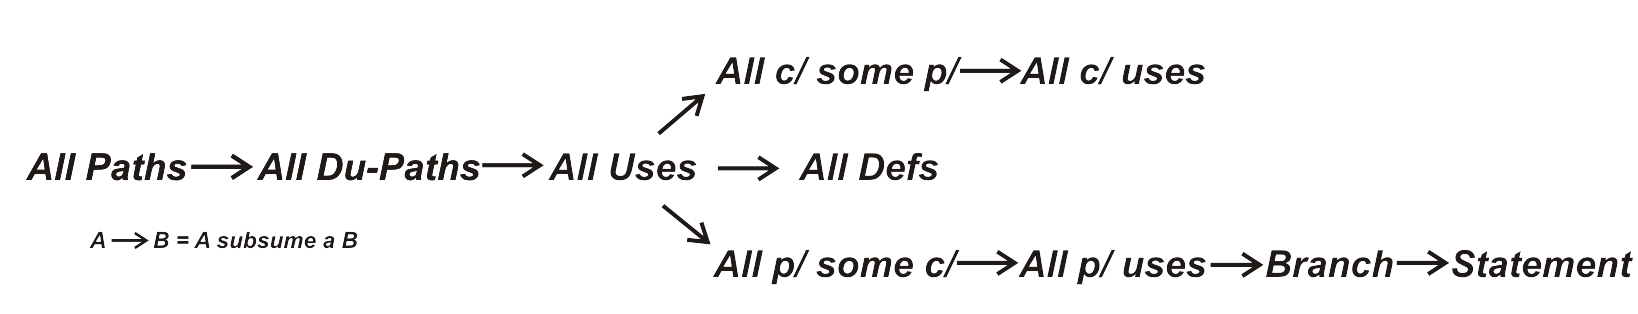
\includegraphics[width = 0.9\textwidth]{Graficos/subsumption.png}

Los de m�s arriba tienen m�s posibilidades de encontrar fallas.

\section{Test de requerimientos no funcionales}
\begin{itemize}
\item Test de seguridad: validando disponibilidad, integridad y confidencialidad de datos y servicios
\item Test de performance: validando los tiempos de acceso y respuesta del sistema
\item Test de stress: validando el uso del sistema en sus l�mites de capacidad y verificando sus reacciones m�s all� de los mismos
\item Test de Usabilidad
\end{itemize}

\section{Ejecuci�n del testing}
\renewcommand{\labelenumi}{\textbf{\alph{enumi}.}}
\begin{enumerate}
	\item \textbf{Selecci�n de datos}
	
Se seleccionan y generan los datos que cumplen con los casos de tests dise�ados para ejecutarlos.

	\item \textbf{Ambiente de test}

El test de unidades se realiza por los programadores en el ambiente de desarrollo, mientras que los tests de aceptaci�n, integraci�n y sistema se realizan en un ambiente de testing separado del de desarrollo. Una vez aceptados, pueden pasar a producci�n, donde son reabsorbidos por desarollo.

	\item \textbf{Terminaci�n del testing}

\begin{itemize}
	\item Se termin� el tiempo o recursos
	\item Se corrieron todos los tests derivados sin detectarse ning�n error
	\item Porcentaje de cubrimiento de ciertas t�cnicas elegidas
	\item Fault-rate m�s bajo que un cierto valor especificado (\# de errores por unidad de tiempo de testing)
	\item Se encontr� un n�mero predeterminado de errores (\% del n�mero total de errores estimado)
\end{itemize}

	\item \textbf{Documentaci�n}

Se deben documentar los casos de test, los criterios utilizados, los datos de prueba y criterios de terminaci�n; tambi�n es necesario un reporte de ejecuci�n luego de haberlos ejecutado que informe del ambiente y los resultados obtenidos.

	\item \textbf{Seguimiento}

Debe realizarse un seguimiento de los errores desde que son detectados hasta que son finalmente aceptados, previo haber pasado por desarrollo para su correcci�n mediante debugging.

	\item \textbf{Test de Regresi�n}

	El test de regresi�n consiste en retestear un sistema luego de haber sido modificado para corregir un determinado elemento, adaptarse a un nuevo ambiente, mejorar prestaciones, etc. Los casos de regresi�n pueden ser:

	\begin{itemize}
		\item Reusables: testeando aspectos no modificados
		\item Restesteables: testeando aspectos de igual especificaci�n pero distinta implementaci�n
		\item Obsoletos: testeando una funcionalidad cuyo requerimiento fue modificado
	\end{itemize}
\end{enumerate}


\clearpage



\end{document}
